\section{The Near Detector Simulation and Reconstruction}\label{sec:nu-osc-06}\label{sec:physics-lbnosc-ND}

% NOTES
% This section must be consistent with the ND executive summary
% Details of the ND as implemented in the LBL analysis are in the appendix
% Section references ArgonCube paper, gas TPC public note
% Need DUNE-PRISM public note, or significant appendix on PRISM
% Need some details on gas TPC analysis in appendix

Oscillation parameters are determined by comparing observed charged-current event spectra at the \dword{fd} to predictions that are, {\em a priori}, subject to uncertainties on the neutrino flux and cross sections at the level of tens of percent as described in the preceding sections. To achieve the required few percent precision of \dword{dune}, it is necessary to constrain these uncertainties with a highly capable \dword{nd} suite. The \dword{nd} is described in detail in \introchnd.

The broad \dword{nd} concept is described briefly in Section~\ref{sec:ndconcept}, along with an outline of the \dword{nd}'s role in the oscillation analysis. The parameterized reconstruction and event selection is described in Section~\ref{sec:ndsimreco}. %More detail can be found in Appendix~\ref{sec:nu-osc-12}. 
\dword{nd} and \dword{fd} uncertainties, including those due to energy estimation and selection efficiencies, are discussed in Section~\ref{sec:physics-lbnosc-syst}.  

\subsection{The Near Detector Concept}
\label{sec:ndconcept}

The \dword{dune} \dword{nd} system consists of a \dword{lartpc} functionally coupled to a magnetized \dword{mpd}, and a \dword{3dst}. The \dword{nd} hall is located at \dword{fnal} 574 m from the neutrino beam source and 60 m underground. The long dimension of the hall is oriented at 90 degrees with respect to the beam axis to facilitate measurements at both on-axis and off-axis locations with a movable detector system. 

The \dword{lartpc} is modular, with fully-\threed  pixelated readout and optical segmentation. These features greatly reduce reconstruction ambiguities that hamper monolithic, projective-readout \dwords{tpc}, and enable the \dword{nd} to function in the high-intensity environment of the \dword{dune} \dword{nd} site. Each module is itself a \dword{lar} \dword{tpc} with two anode planes and a central cathode. The active dimensions of each module are $1 \times 3 \times 1$~m ($x \times y \times z$), where the $z$ direction is $6^{\circ}$ upward from the neutrino beam, and the $y$ direction points upward. Charge drifts in the $\pm x$ direction, with a maximum drift distance of 50 cm for ionization electrons produced in the center of a module. The module design is described in detail in Ref.~\cite{Asaadi:2018xfh}. The full \dword{lar} detector consists of an array of modules in a single cryostat. The minimum active size for full containment of hadronic showers is $3 \times 4 \times 5$~m. High-angle muons can also be contained by extending the width to 7 m. For this analysis, 35 modules are arranged in an array 5 modules deep in the $z$ direction and 7 modules across in $x$ so that the total active dimensions are $7 \times 3 \times 5$~m. The total active \dword{lar} volume is $105$~m$^{3}$, corresponding to a mass of 147 tons.

The anode planes are tiled with readout pads, such that the $yz$ coordinate is given by the pad location and the $x$ coordinate is given by the drift time, and the three-dimensional position of an energy deposit is uniquely determined. A dedicated, low-power readout ASIC is being developed, which will enable single-pad readout without analog multiplexing~\cite{Dwyer:2018phu}. The module walls orthogonal to the anode and cathode are lined with a photon detector that is sensitive to scintillation light produced inside the module, called ArCLight~\cite{Auger:2017flc}. The detector is optically segmented, and tiled so that the vertical position of the optical flash can be determined with $\sim$30 cm resolution. It is therefore possible to isolate flashes to a volume of roughly 0.3 m$^{3}$, and associate them to a specific neutrino interaction even in the presence of pile-up. The neutrino interaction time, $t_{0}$, is determined from the prompt component of the scintillation light.

The \dword{mpd} consists of a high-pressure \dword{gartpc} in a cylindrical pressure vessel at 10 bar, surrounded by a granular, high-performance electromagnetic calorimeter. The \dword{mpd} sits immediately downstream of the \dword{lar} cryostat so that the beam center crosses the exact center of both the \dword{lar} and gaseous argon active volumes. The pressure vessel is 5 m in diameter and 5 m long. The \dword{tpc} is divided into two drift regions by a central cathode, and filled with a 90/10 Ar/CH$_{4}$ gas mixture, such that 97\% of neutrino interactions will occur on the Ar target. The gas TPC is described in detail in Ref.~\cite{bib:docdb12388}.

The electromagnetic calorimeter is composed of a series of absorber layers followed by arrays of scintillator read out by SiPMs mounted directly onto boards. The inner-most layers will be tiled, giving \threed position information for each hit, and sufficient granularity to enable reconstruction of the angle of incoming photons. The \dword{ecal} design is described in Ref. ~\cite{Emberger:2018pgr}. The entire \dword{mpd} sits inside a magnetic field with a strength of at least 0.4 T. A superconducting magnet is preferred, to reduce the total amount of mass near the detectors.

The optimization of the detector design is still underway at the time of preparing this document, and the eventual parameters may be somewhat different from what is simulated. For the oscillation analysis presented herein, only the \dword{lar} event sample is explicitly used. The \dword{ecal}, pressure vessel, and magnet design have a small impact on the acceptance of muons originating in the \dword{lar}. The \dword{ecal} is assumed to be 30 layers of alternating planes of 5mm CH and 2mm Cu. The pressure vessel is assumed to be 3 cm thick titanium. The magnet is a solenoid with an inner radius of 320 cm, with a yoke cut out of the upstream barrel to minimize the passive material between the two \dword{tpc} detectors. The \dword{3dst} is not functionally coupled to the \dword{lar} detector and thus is not included in these simulations. Small changes in these parameters are not expected to significantly impact the acceptance. A profile view visualization of the ND as implemented in this analysis is shown in Figure~\ref{fig:NDvis}.
%For the oscillation sensitivity analysis presented in this document, the pressure vessel is assumed to be 3 cm titanium. The ECAL tiles are $10 \times 10 \times 5$~mm, with a 2 mm copper absorber. The inner-most 10 ECal layers are inside the pressure vessel, giving excellent angular resolution to photon-induced showers, which generally do not convert in the gas. An additional 20 ECal layers are positioned outside the pressure vessel to contain energy from these showers. The magnet is a solenoid with an inner radius of 320 cm and total length along the cylinder axis of 780 cm. The yoke is cut out in the upstream barrel to minimize the passive material between the two TPC detectors. A profile view visualization of the ND is shown in Figure~\ref{fig:NDvis}.

\begin{dunefigure}[ND visualization]{fig:NDvis}
{The near detector shown from the side. The neutrinos are incident from the left along the axis shown, which intersects the center of the LAr and GAr detectors.}
 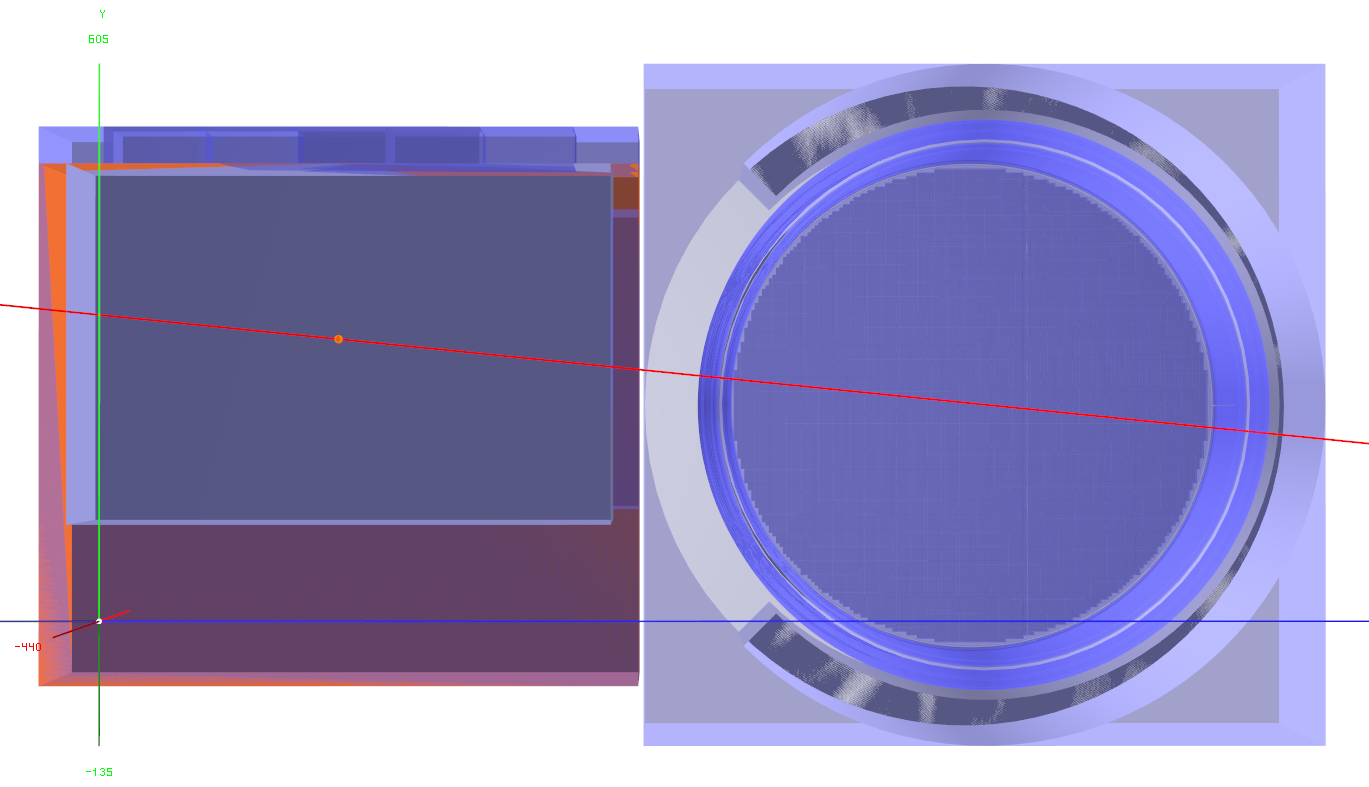
\includegraphics[width=0.6\textwidth]{lar_mpt_in_hall.png}
\end{dunefigure}

The oscillation analysis includes samples of $\nu_{\mu}$ and $\bar{\nu}_{\mu}$ charged-current interactions originating in the \dword{lar}. The samples are binned in \twod as a function of neutrino energy and inelasticity, $y = 1 - E_{\mu}/E_{\nu}$, where $E_{\mu}$ and $E_{\nu}$ are the muon and neutrino energies, respectively. 

\subsection{Event Simulation and Parameterized Reconstruction}
\label{sec:ndsimreco}

Neutrino interactions are simulated in the active volumes of the \dword{lar} and \dword{hpg} \dwords{tpc}. The neutrino flux prediction is described in Section~\ref{sec:physics-lbnosc-flux}. Interactions are simulated with the \dword{genie} event generator using the model configuration described in Section~\ref{sec:nu-osc-05}. The propagation of neutrino interaction products through the detector volumes is simulated using a \dword{geant4}-based model. Pattern recognition and reconstruction software has not yet been developed for the \dword{nd}. Instead, we perform a parameterized reconstruction based on true energy deposits in active detector volumes as simulated by \dword{geant4}.

\subsubsection{Liquid Argon charged-current interactions}

Liquid argon events are required to originate in a fiducial volume that excludes 50 cm from the sides and upstream edge, and 150 cm from the downstream edge of the active region, for a total of $6 \times 2 \times 3$~m$^{2}$. A hadronic veto region is defined as the outer 30 cm of the active volume on all sides. Events with more than 30 MeV total energy deposit in the veto region are excluded from analysis, as this energy near the detector edge suggests leakage, resulting in poor energy reconstruction. Even with the containment requirement, events with large shower fluctuations to neutral particles can still be very poorly reconstructed. Neutrons, in particular, are largely unreconstructed energy.

Electrons are reconstructed calorimetrically in the liquid argon. The radiation length is 14 cm in \dword{lar}, so for fiducial interactions and forward-going electrons there are between 10 and 30 radiation lengths between the vertex and the edge of the \dword{tpc}. As there is no magnetic field in the \dword{lar} \dword{tpc} region, electrons and positrons cannot be distinguished and the selected $\nu_{e}$ sample contains both neutrino- and antineutrino-induced events.

Muons with kinetic energy greater than $\sim$1 GeV typically exit the \dword{lar}. An energetic forward-going muon will pass through the ECal and into the gaseous \dword{tpc}, where its momentum and charge are reconstructed by curvature. For these events, it is possible to differentiate between $\mu^{+}$ and $\mu^{-}$ event by event. Muons that stop in the \dword{lar} or ECal are reconstructed by range. Exiting muons that do not match to the \dword{hpg} \dword{tpc} are not reconstructed, and events with these tracks are rejected from analysis.
%Events with exiting tracks that do not enter the \dword{hpg} \dword{tpc} are rejected. 
These are predominantly muon CC, where the muon momentum cannot be determined. Forward exiting muons will enter the magnetized \dword{mpd}, where their momenta and charge sign are reconstructed by curvature. The asymmetric transverse dimensions of the \dword{lar} volume make it possible to reconstruct wide-angle muons with some efficiency. High-angle tracks are typically lost when the $\nu-\mu$ plane is nearly parallel to the $y$ axis, but are often contained when it is nearly parallel to the $x$ axis. 

The charge of stopping muons in the \dword{lar} volume cannot be determined. However, the wrong-sign flux is predominantly concentrated in the high-energy tail, where leptons are likelier to be forward and energetic. In FHC mode, the wrong-sign background in the focusing peak is negligibly small, and $\mu^{-}$ is assumed for all stopping muon tracks. In RHC mode, the wrong-sign background is larger in the peak region. Furthermore, high-angle leptons are generally at higher inelasticity, $y$, which enhances the wrong-sign contamination in the contained muon subsample. To mitigate this, a Michel electron is required. The wrong-sign $\mu^{-}$ captures on Ar with 75\% probability, effectively suppressing the relative $\mu^{-}$ component by a factor of four.

Events are classified as either $\nu_{\mu}$ CC, $\bar{\nu}_{\mu}$ CC, $\nu_{e}$+$\bar{\nu}_{e}$ CC, or NC. True muons and charged pions are evaluated as potential muon candidates. The track length is determined by following the true particle trajectory until it hard scatters or ranges out. The particle is classified as a muon if its track length is at least 1 m, and the mean energy deposit per centimeter of track length is less than 3 MeV. The mean energy cut rejects tracks with detectable hadronic interactions. The minimum length requirement imposes an effective threshold on true muons of about 200 MeV kinetic energy, but greatly suppresses potential NC backgrounds with short, non-interacting charged pions.

True electrons are reconstructed with an ad-hoc efficiency that is zero below 300 MeV, and rises linearly to unity between 300 and 700 MeV. Neutral-current backgrounds arise from photon and $\pi^{0}$ production. Photons are misreconstructed as electrons when the energy deposit per centimeter in the first few cm after conversion is less than 4 MeV. This is typically for Compton scatters, and can also occur due to a random downward fluctuation in the $e^{+}e^{-}$ dE/dx. The conversion distance must also be small so that no visible gap can be identified. We consider a photon gap to be clear when the conversion distance is greater than 2 cm, which corresponds to at least four pad widths. For $\pi^{0}$ events, the second photon must also be either less than 50 MeV, or have an opening angle to the first photon less than 10 mrad. Electrons are generally contained in the \dword{lar} and are reconstructed calorimetrically. It is possible for CC $\nu_{\mu}$ events to be reconstructed as CC $\nu_{e}$ when the muon is too soft and a $\pi^{0}$ fakes the electron.

\dword{lar} events are classified as $\nu_{\mu}$ CC, $\bar{\nu}_{\mu}$ CC, $\nu_{e}$ + $\bar{\nu}_{e}$ CC, or NC. Charged-current events are required to have exactly one reconstructed lepton of the appropriate flavor. The muon-flavor samples are separated by reconstructed charge, but the electron-flavor sample is combined because the charge cannot be determined. The neutral-current sample includes all events with zero reconstructed leptons. Spectra for selected \numu \dword{cc} events in \dword{fhc} are shown in Figure~\ref{fig:recoSamples} as a function of both neutrino energy and inelasticity.

\begin{dunefigure}[ND selected samples]{fig:recoSamples}
{Reconstructed neutrino energy and $y$ for events classified as $\nu_{\mu}$ \dword{cc} in \dword{fhc} mode. Background events are predominantly neutral currents and are shown in red.}
 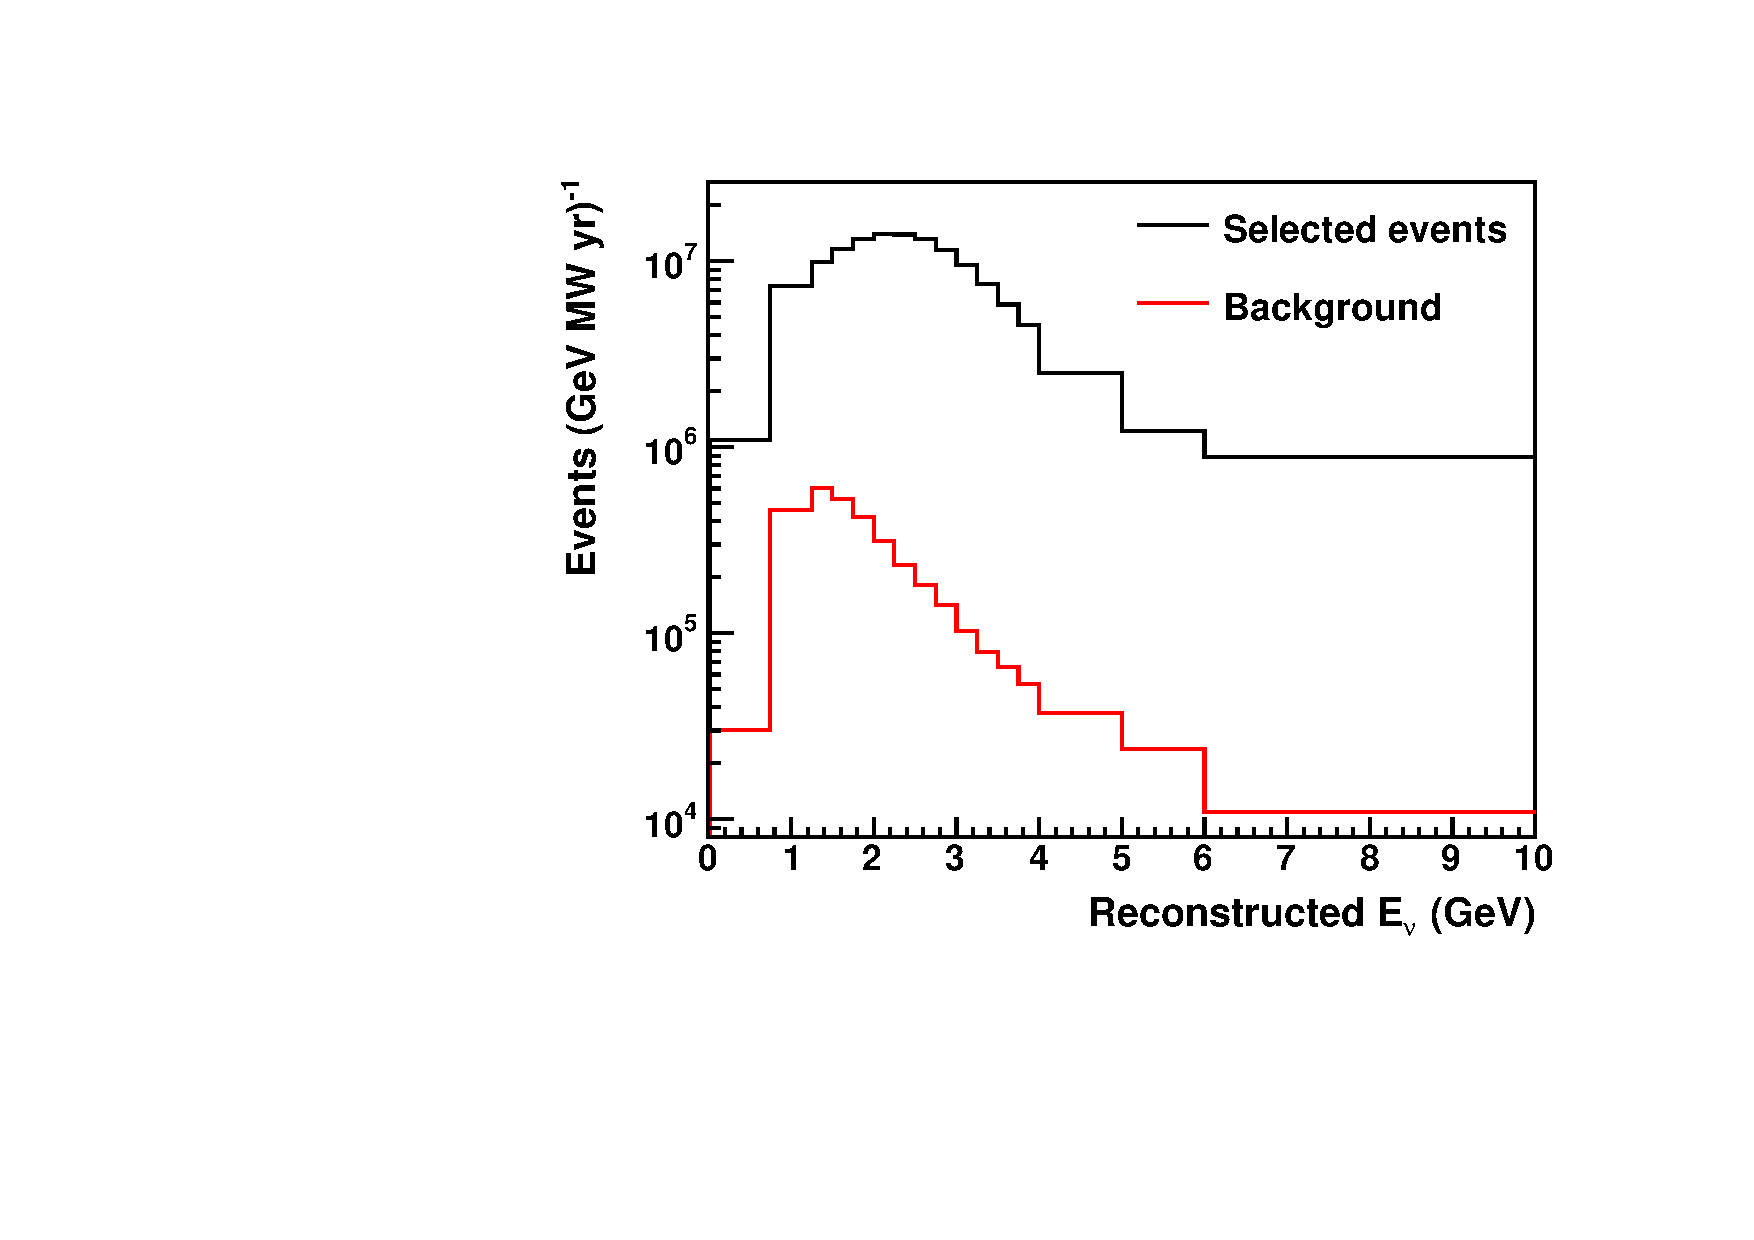
\includegraphics[width=0.48\textwidth]{FHC_selected_Ev_log.pdf}
 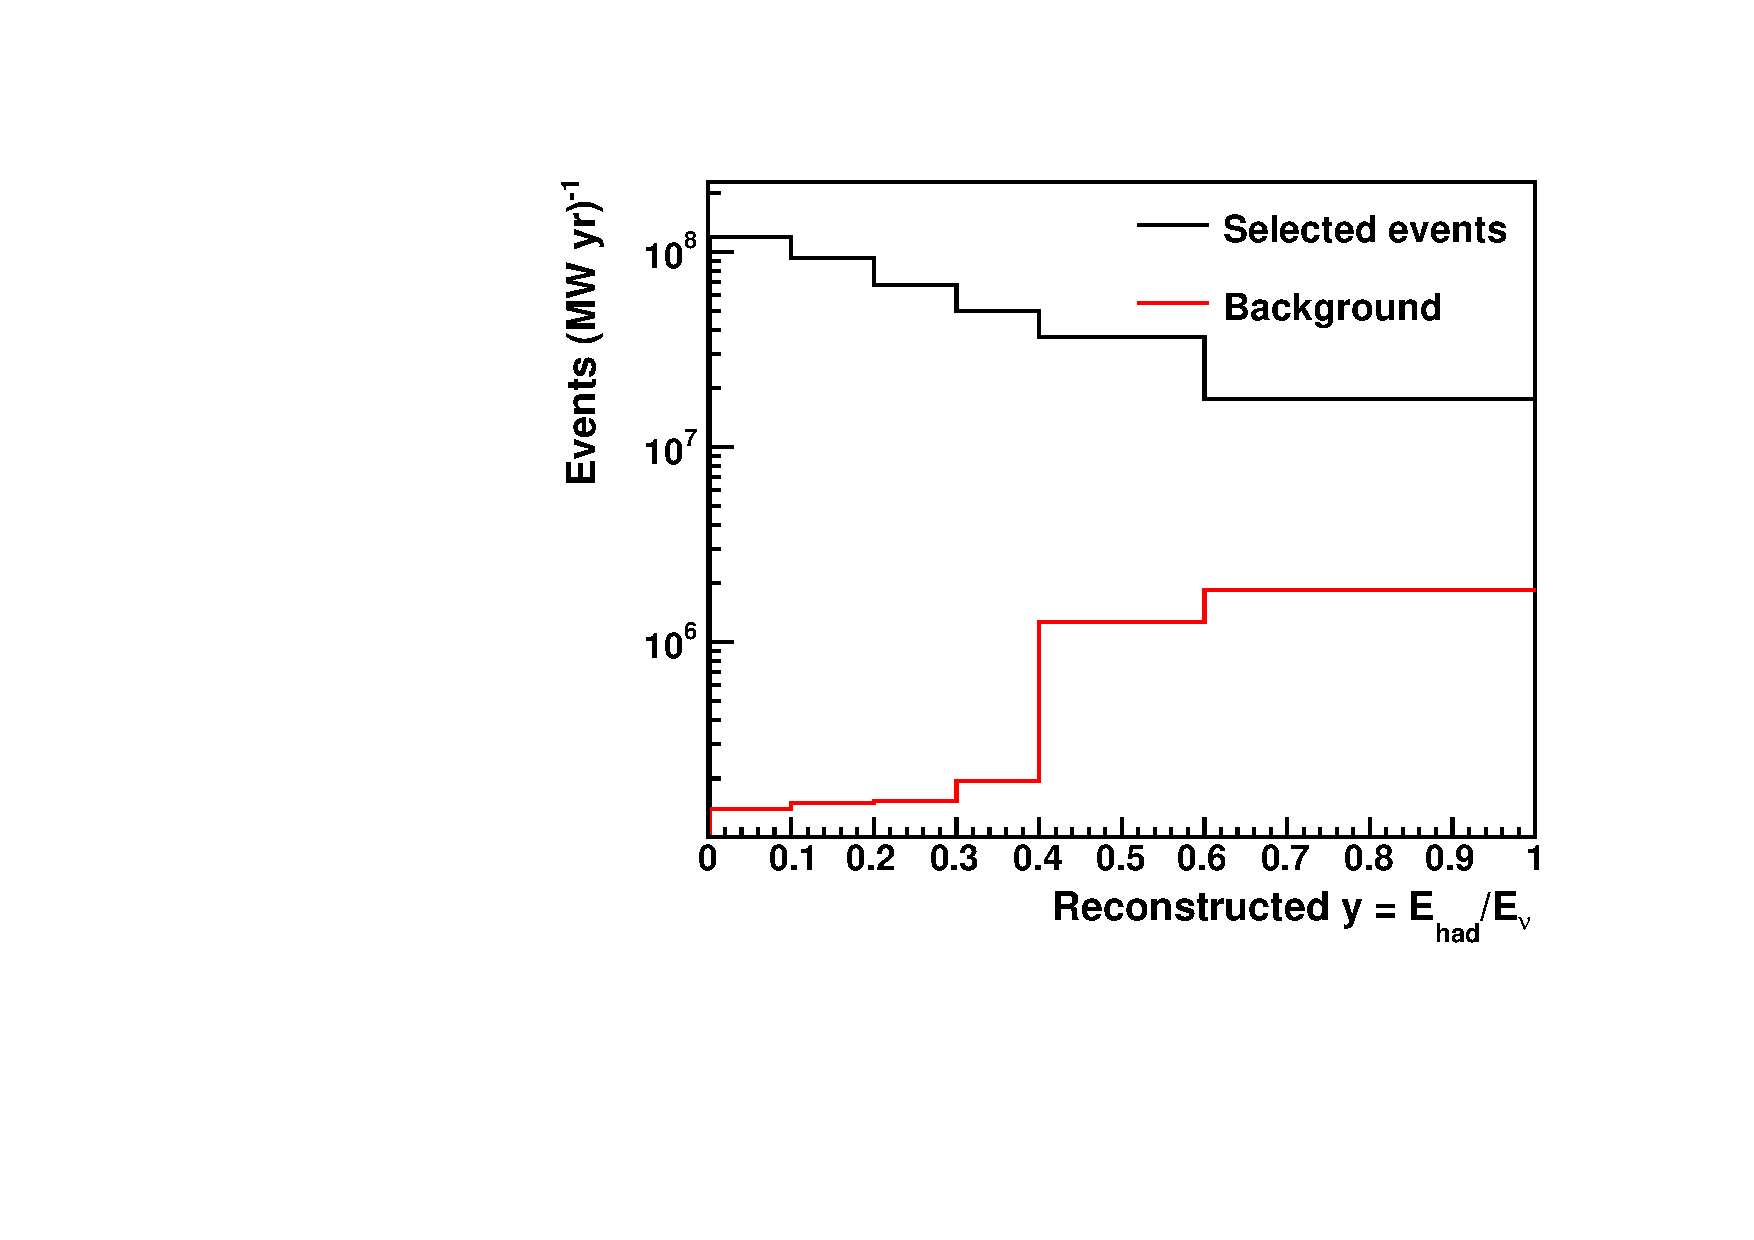
\includegraphics[width=0.48\textwidth]{FHC_selected_y_log.pdf}
\end{dunefigure}

Hadronic energy is estimated by summing visible energy deposits in the active \dword{lar} volume. Events are rejected when energy is observed in the outer 30 cm of the detector, which is evidence of poor hadronic containment.  Events with more than 30 MeV of visible hadronic energy in the veto region are also excluded.  This leads to an acceptance that decreases with hadronic energy, as shown in the right panel of Figure~\ref{fig:NDacceptance}.

% Muons are contained up to kinetic energies of $\sim$1 GeV, above which they typically exit the detector.  The acceptance is somewhat lower at large angles, as shown in the center panel of Figure~\ref{fig:NDreco}.

Events are classified as either $\nu_{\mu}$ \dword{cc}, $\bar{\nu}_{\mu}$ \dword{cc}, $\nu_{e}$+$\bar{\nu}_{e}$ \dword{cc}, or \dword{nc} based on the presence of charged leptons. Backgrounds to $\nu_{\mu}$ \dword{cc} arise from \dword{nc} $\pi^{\pm}$ production where the pion leaves a long track and does not shower. Muons below about 400 MeV kinetic energy have a significant background from charged pions, so these \dword{cc} events are excluded from the selected sample. Backgrounds to $\nu_{e}$ \dword{cc} arise from photons that convert very near the interaction vertex. The largest contribution is from $\pi^{0}$ production with highly asymmetric decay.

\begin{dunefigure}[ND acceptance]{fig:NDacceptance}
{Left: Detector acceptance for $\nu_{\mu}$ \dword{cc} events as a function of muon transverse and longitudinal momentum. Right: Acceptance as a function of hadronic energy; the black line is for the full fiducial volume while the red line is for a $1 \times 1 \times 1$~m$^{3}$ volume in the center, and the blue curve is the expected distribution of hadronic energy given the \dword{dune} flux.}
 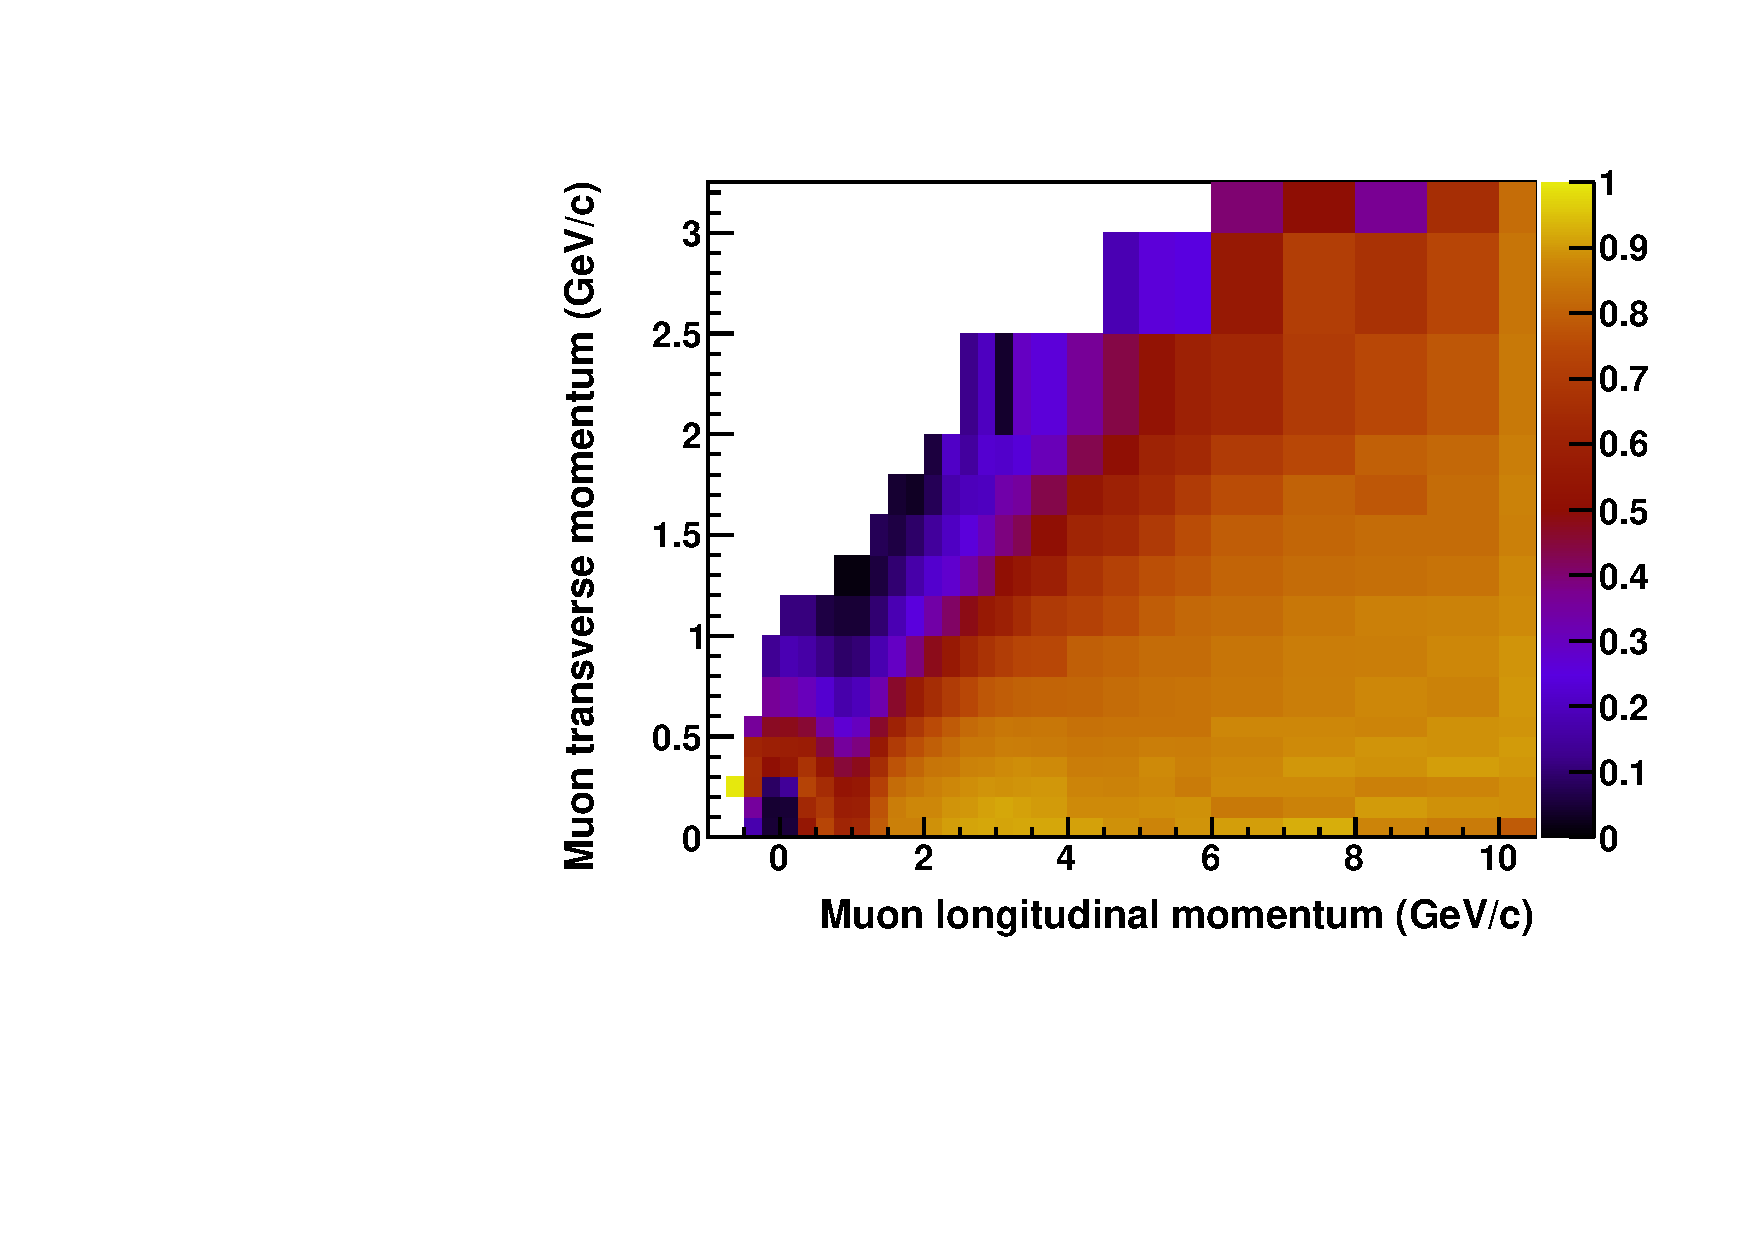
\includegraphics[width=0.48\textwidth]{pL_pT_eff.pdf}
 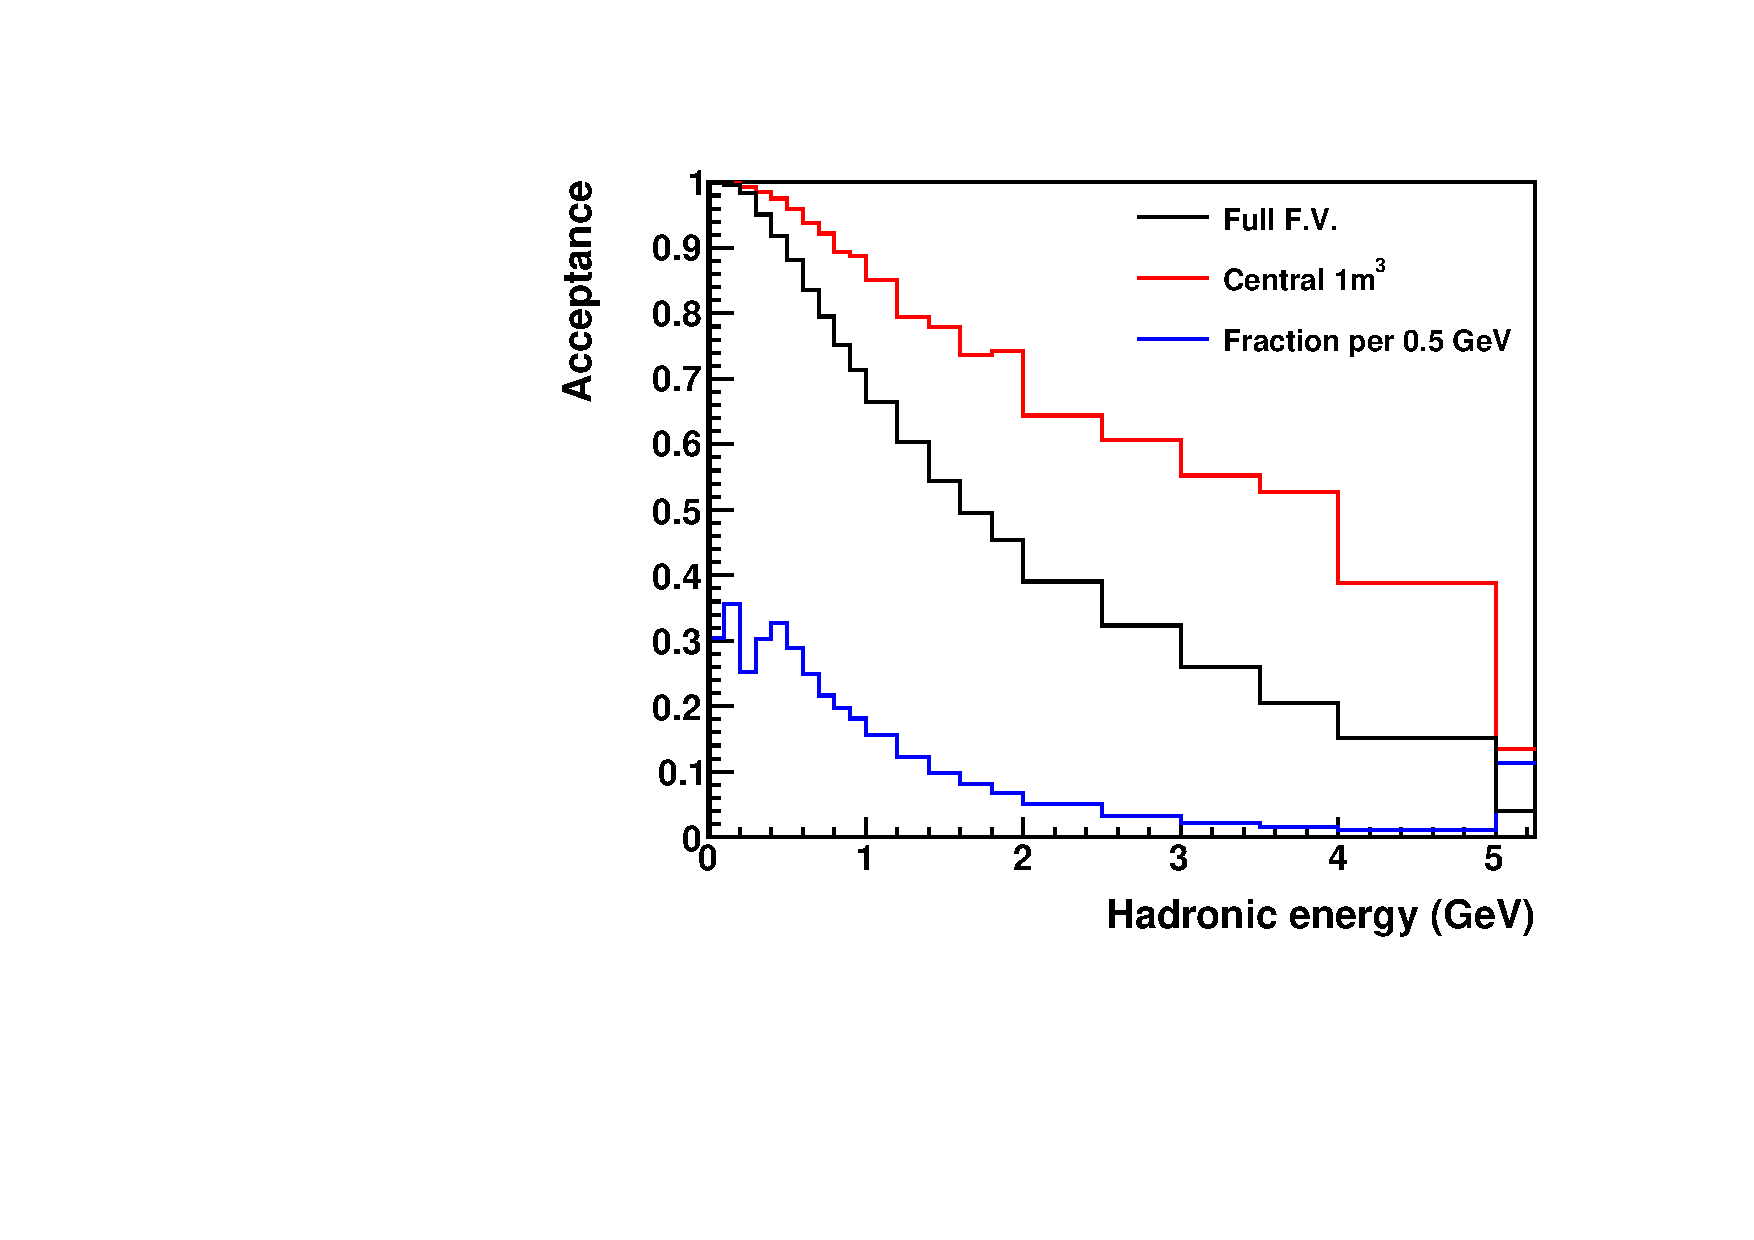
\includegraphics[width=0.48\textwidth]{Ehad_eff.pdf}
\end{dunefigure}

\subsubsection{Neutrino-electron elastic scattering}

%Neutrino-electron scattering is a pure-electroweak process with calculable cross section at tree level. It is therefore possible to directly constrain the flux by measuring the event rate of $\nu+ e \rightarrow \nu +e$ and dividing by the known cross section. The two-body elastic process is subject to the kinematic constraint $E_{e}\theta_{e}^{2} < 2m_{e}$, where $E_{e}$, $\theta_{e}$, and $m_{e}$ are the final-state electron energy, angle, and mass, respectively.

%The \dword{lartpc} has sufficient energy and angular resolution to separate the signal, peaked at low $E_{e}\theta_{e}^{2}$, from backgrounds due to $\nu_{e}$ \dword{cc} scattering and from \dword{nc} $\pi^{0}$ production. The expected rate is \num{3300} events per year, so that the statistical uncertainty on the absolute flux normalization can be constrained to $\sim$1\% with three years of running. The dominant systematic uncertainty is expected to be the $\nu_{e}$ \dword{cc} shape at low $Q^{2}$, and can be constrained with sidebands to the $\sim$1\% level so that the overall uncertainty is $\sim$2\%.

In addition to the CC event selections, neutrino-electron elastic scattering is also selected. Measurements of neutrino-nucleus scattering are sensitive to the product of the flux and cross section, both of which are uncertain. This can lead to a degeneracy between flux and cross section nuisance parameters in the oscillation fit, and result in significant anti-correlations, even when the uncertainty on the diagonal component is small. One way to break this degeneracy is by including a sample for which the a priori cross section uncertainties are very small. 

Neutrino-electron scattering is a pure-electroweak process with calculable cross section. It is therefore possible to directly constrain the flux by measuring the event rate of $\nu+ e \rightarrow \nu +e$ and dividing by the known cross section. The final state consists of a single electron, subject to the kinematic limit 

\begin{equation}
1 - \cos \theta = \frac{m_{e}(1-y)}{E_{e}},
\end{equation}

where $\theta$ is the angle between the electron and incoming neutrino, $E_{e}$ and $m_{e}$ are the electron mass and total energy, respectively, and $y = T_{e}/E_{\nu}$ is the fraction of the neutrino energy transferred to the electron. For DUNE energies, $E_{e} \gg m_{e}$, and the angle $\theta$ is very small, such that $E_{e}\theta^{2} < 2m_{e}$.

The overall flux normalization can be determined by counting $\nu e \rightarrow \nu e$ events. Events can be identified by searching for a single electromagnetic shower with no other visible particles. Backgrounds from $\nu_{e}$ charged-current scattering can be rejected by looking for large energy deposits near the interaction vertex, which are evidence of nuclear breakup. Photon-induced showers from neutral-current $\pi^{0}$ events can be distinguished from electrons by the energy profile at the start of the track. The dominant background is expected to be $\nu_{e}$ charged-current scattering at very low $Q^{2}$, where final-state hadrons are below threshold, and $E_{e}\theta^{2}$ happens to be small. The background rate can be constrained with a control sample at higher $E_{e}\theta^{2}$, but the shape extrapolation to $E_{e}\theta^{2} \rightarrow 0$ is uncertain at the 10-20\% level.

For the DUNE flux, approximately 100 events per year per ton of fiducial mass are expected with electron energy above 0.5 GeV. For a LAr TPC mass of 25 tons, this corresponds to 2500 events per year, or 12500 events in the full 5-year FHC run, assuming the ND stays on axis. Given the very forward signal, it may be possible to expand the fiducial volume to enhance the rate. The statistical uncertainty on the flux normalization from this technique is expected to be $\sim$1\%.

To evaluate the impact of neutrino-electron scattering, a dedicated high-statistics signal-only sample is generated. Due to the simple nature of the signal, it is possible to estimate backgrounds without a full detector simulation. A single electromagnetic shower (electron, positron or photon) is required. To reject $\pi^{0}$ events with clearly-identifiable second photons, no additional showers over 50 MeV are allowed.

Charged-current $\nu_{e}$ interactions can be rejected when there is evidence of nuclear breakup in the form of final-state charged hadrons. A conservative cut of 40 MeV total charged hadron kinetic energy is applied. For a single proton, this corresponds to $\sim$ 1 cm of track length, which will leave energy on two or three readout pads and be easily identified. Finally, a cut requiring low $E_{e}\theta_{e}^{2}$ isolates the $\nu+e$ signal. Alternatively, templates in $(E_{e}, \theta_{e})$ can be formed, and the unique shape of the signal can be used in a fit to extract the flux normalization.

\subsubsection{Off-axis \dword{nd} measurements}
\label{sec:ch-nu-osc-06-ndconcept-offaxis}

Neutrino energy reconstruction is one of the biggest challenges in a precision long-baseline oscillation experiment like \dword{dune}. Even with a highly capable \dword{fd}, a fraction of the final-state hadronic energy is typically not observed. For example, neutrons may travel meters without interacting, and can exit the detector with significant kinetic energy. This missing energy is typically corrected with a neutrino interaction generator, which is used to relate the true neutrino energy to the observed energy. These models have many tens of uncertain parameters, which can be constrained by \dword{nd} measurements. However, there may be many different parameter combinations that adequately describe the \dword{nd} data. These degenerate solutions can extrapolate differently to the \dword{fd}, where the flux is significantly different due to oscillations. This can lead to biases in the fitted oscillation parameters, including $\delta_{CP}$, despite an apparently good quality of fit.

While these biases can be partially mitigated by an on-axis \dword{nd} capable of making numerous exclusive measurements, the energy dependence of the interaction cross section and the bias in reconstructed neutrino energy cannot be measured in a single beam. To gain sensitivity to these, the \dword{lartpc} and \dword{mpd} combination is movable, and the \dword{nd} hall is oriented to facilitate both on-axis measurements and measurements at positions up to 33 m off axis. The flux spectrum varies as a function of off-axis angle, peaking lower in energy as the angle is increased, as shown in Figure~\ref{fig:OAAFluxFigs}. As uncertainties in the flux prediction are strongly correlated across off-axis angles, off-axis measurements of reconstructed neutrino energy constrain cross section uncertainties and provide further handles on possible degeneracies in the fit. By taking linear combinations of such measurements, it is also possible to reproduce the predicted \dword{fd} oscillated flux for some set of oscillation parameters, and directly compare visible energy between \dword{nd} and \dword{fd} over essentially the same "oscillated" flux, and with greatly reduced model dependence. Figure~\ref{fig:nd_prism} shows the result of such a linear combination, overlaid with the \dword{fd} flux. The off-axis technique cannot reproduce the \dword{fd} flux tail. The lower $E_{\nu}$ bound is determined by the range of accessible off-axis angles; to cover down to 0.5 GeV, measurements out to 33 m off axis are required.

\begin{dunefigure}[DUNE-PRISM fluxes]{fig:nd_prism}
{The predicted \dword{fd} flux (black), and a prediction made up of linear combinations of \dword{nd} fluxes (green).}
 % Possibly include figure from mock data study here
 %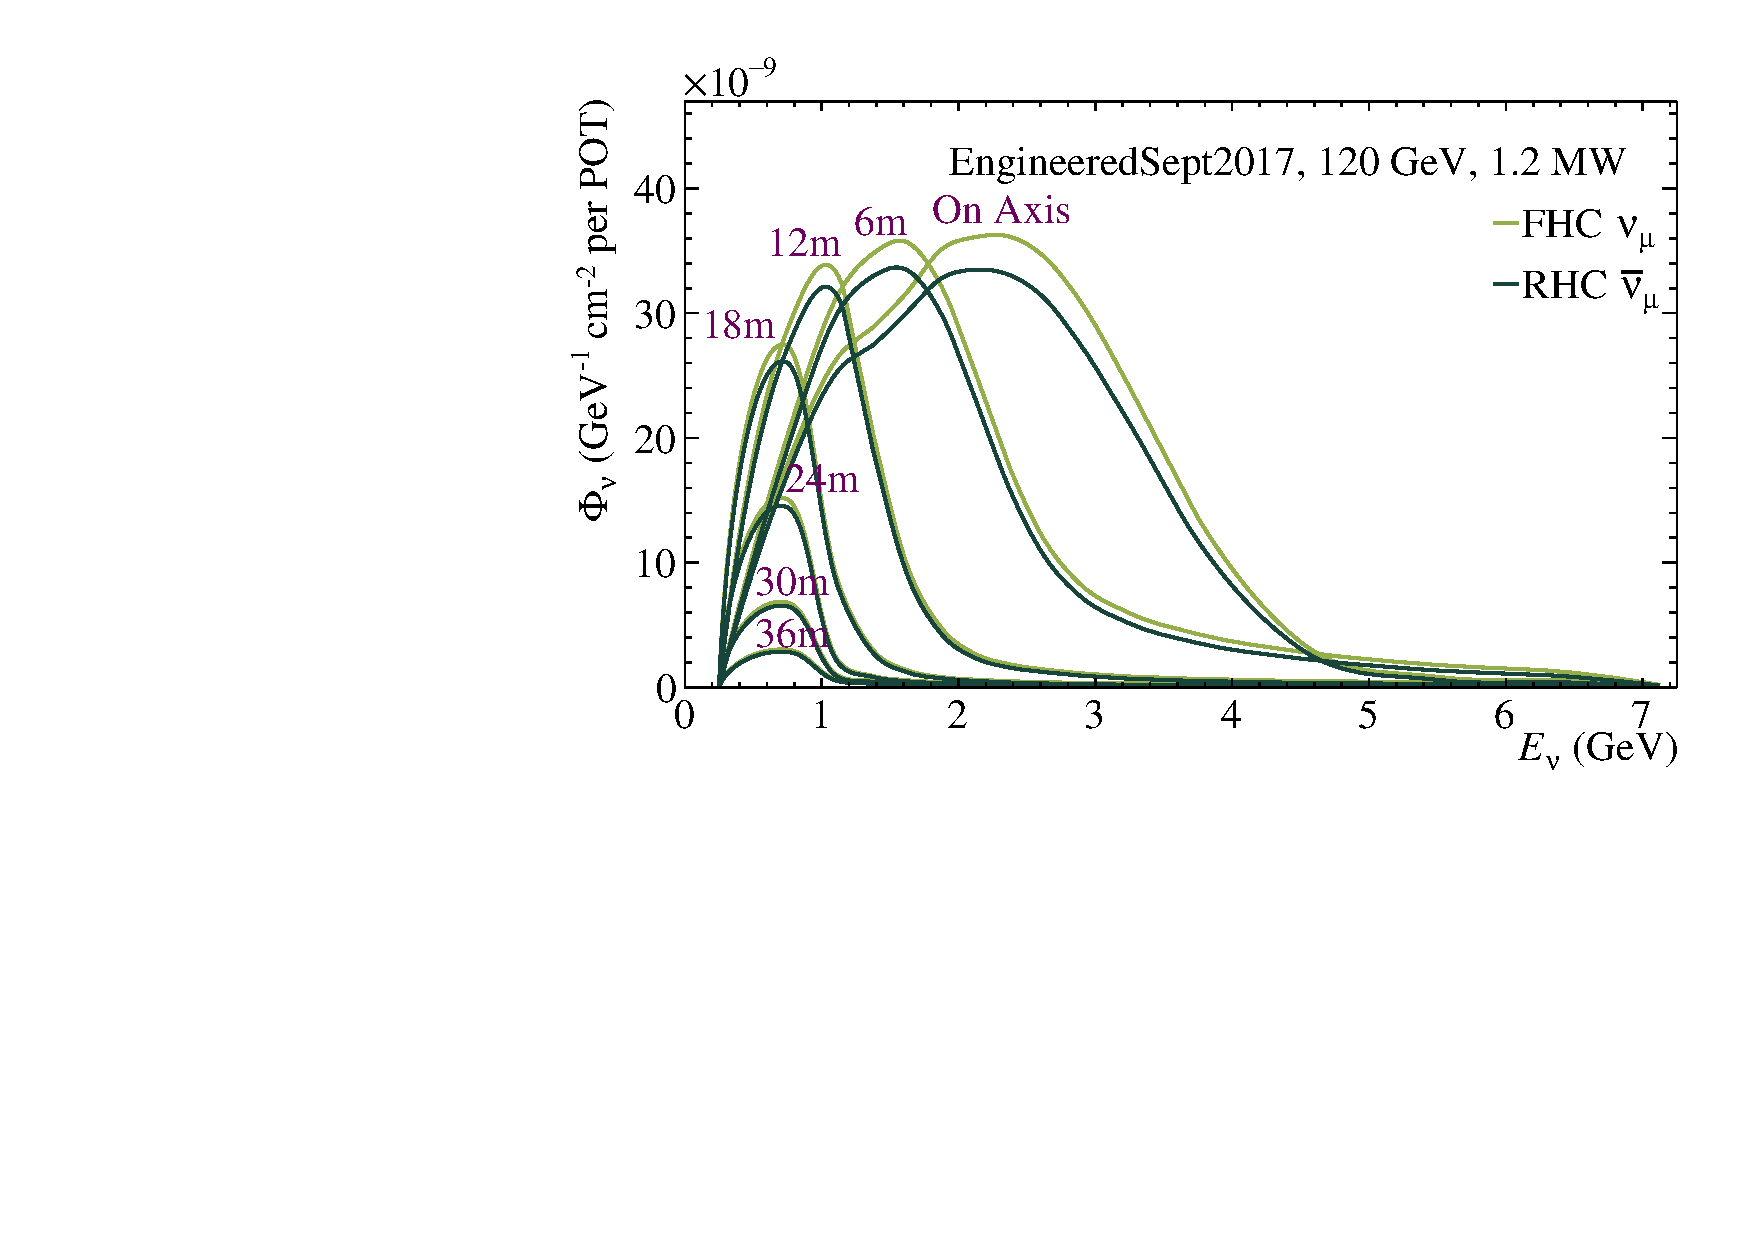
\includegraphics[width=0.49\textwidth]{graphics/OffAxisFluxes_1D.pdf}
 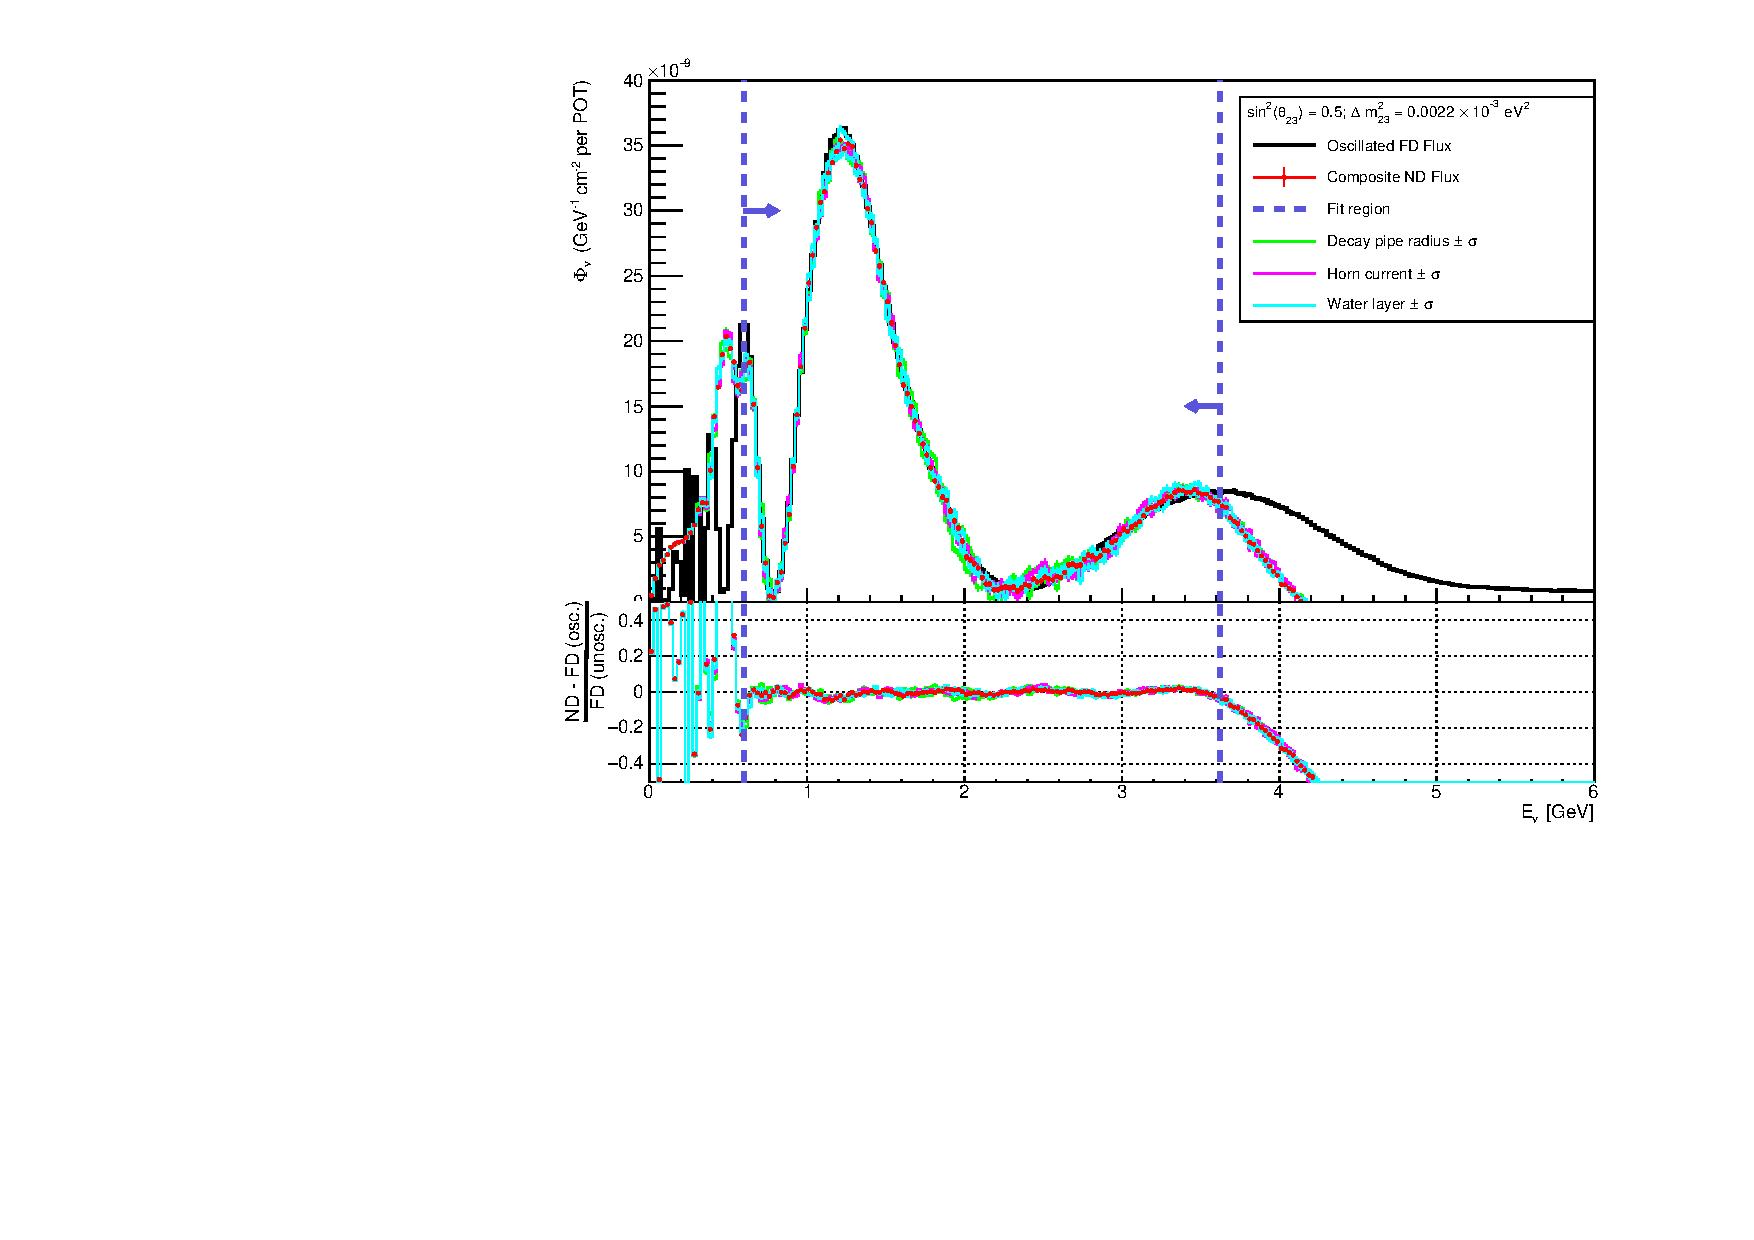
\includegraphics[width=0.49\textwidth]{nuprism_coef_oscSpectrum_0_0022_0_5.pdf}
\end{dunefigure}

A potential run plan is to take on-axis data approximately 50\% of the time, with the other 50\% split among enough off-axis positions so that the fiducial volumes of adjacent ``stops'' overlap, giving a continuous range of angles. Event selection at an off-axis location of the \dword{lar} detector is identical to the on-axis case. The selection efficiency varies as a function of muon energy due to containment and matching to the downstream magnetized tracker, and as a function of hadronic energy due to containment. As muon and hadronic energy are correlated to neutrino energy, the efficiency varies with off-axis position. The efficiency also varies as a function of vertex position; interactions occurring near the edges of the detector are more likely to fail containment requirements. These effects are corrected with simulation; as they are largely geometric, the uncertainties that arise from the corrections are small compared to the uncertainties on neutrino cross sections and energy reconstruction. %More details on the off-axis analysis are found in Appendix~\ref{sec:physics-lbnosc-ND-app}.

\subsubsection{Gaseous argon charged-current interactions}

With over 30 million charged-current events per year, the \dword{lartpc} event sample can be analyzed in many different exclusive channels and provide powerful constraints. However, its relatively high density makes certain hadronic topologies challenging to reconstruct. The gaseous \dword{tpc} complements the \dword{lar} detector by providing low reconstruction thresholds, excellent pion/proton separation, and charge-sign reconstruction. In particular, measurements of proton and charged pion multiplicities as a function of neutrino energy constrain cross section uncertainties not accessible to the \dword{lar} alone.

In addition, the gas \dword{tpc} provides a useful check on the reconstruction efficiency of the \dword{lar} selection. Due to the combining of contained muons with gas \dword{tpc}-matched events, there are kinematic regions where the acceptance of the \dword{lartpc} is uncertain. Also, without a magnetic field, the wrong sign contamination cannot be directly measured, especially at high angle and low energy. The gas \dword{tpc}, however, has uniform acceptance over the full 4$\pi$, as well as charge measurement capability except when the muon is nearly parallel to the magnetic field lines.

Unlike the \dword{lartpc}, where the hadronic energy is determined by a calorimetric sum of energy deposits, the gas \dword{tpc} hadronic energy is reconstructed particle-by-particle, including pion masses. For this analysis, samples of $\nu_{\mu}$ \dword{cc} events are selected in slices of charged pion multiplicity, and fit as a function of reconstructed neutrino energy. The threshold for charged pion selection is 5 MeV, and $\pi^{+}$ can be reliably separated from protons up to momenta of 1.3 GeV/c.

%\subsection{Use of near detector in oscillation analysis}

